\chapter{The Large Hadron Collider}

\section{Experimental Apparatus}

The Large Hadron Collider (LHC) is a circular proton-proton collider, 27 km in circumference and between 40 and 175 m below the surface, located at the European Organization for Nuclear Research (CERN) on the French-Swiss border near the city of Geneva~\cite{Evans2008}.
Designed to collide protons at a maximum center-of-mass energy $\sqrt{s} = 14\TeV$, the LHC has delivered collisions at $\sqrt{s} = 7, 8 \TeV$ during Run 1 (2010-2012) and at $\sqrt{s} = 13\TeV$ during Run 2 (2015-2018).
While the LHC is primarily a proton-proton collider, lead (Pb) ion beams of energy of up to 2.8 TeV per nucleon are used to produce lead-lead and proton-lead collisions.
In this thesis, we focus exclusively on data recorded from proton-proton collisions during Run 2.

The LHC is the final stage of the CERN accelerator complex~\cite{Benedikt2004} depicted in Figure~\ref{fig:lhc}.
Hydrogen atoms are stripped of their electrons and accelerated to an energy of 50\MeV by the LINAC2 linear acceleration.
Following this, they are injected into the Booster ring, the Proton Synchrotron (PS), and the Super Proton Synchrotron (SPS) and accelerated to 1.4, 26, and 450\GeV, respectively.
After the SPS, the protons are injected into the two counter-circulating rings of the LHC in up to 2808 discrete bunches with a bunch spacing of 25\ns.
The two beams intersect in eight places along the LHC with detector experiments CMS, ATLAS, LHCb, and ALICE each located at an intersection point.

\begin{figure}[htbp]
  \centering
  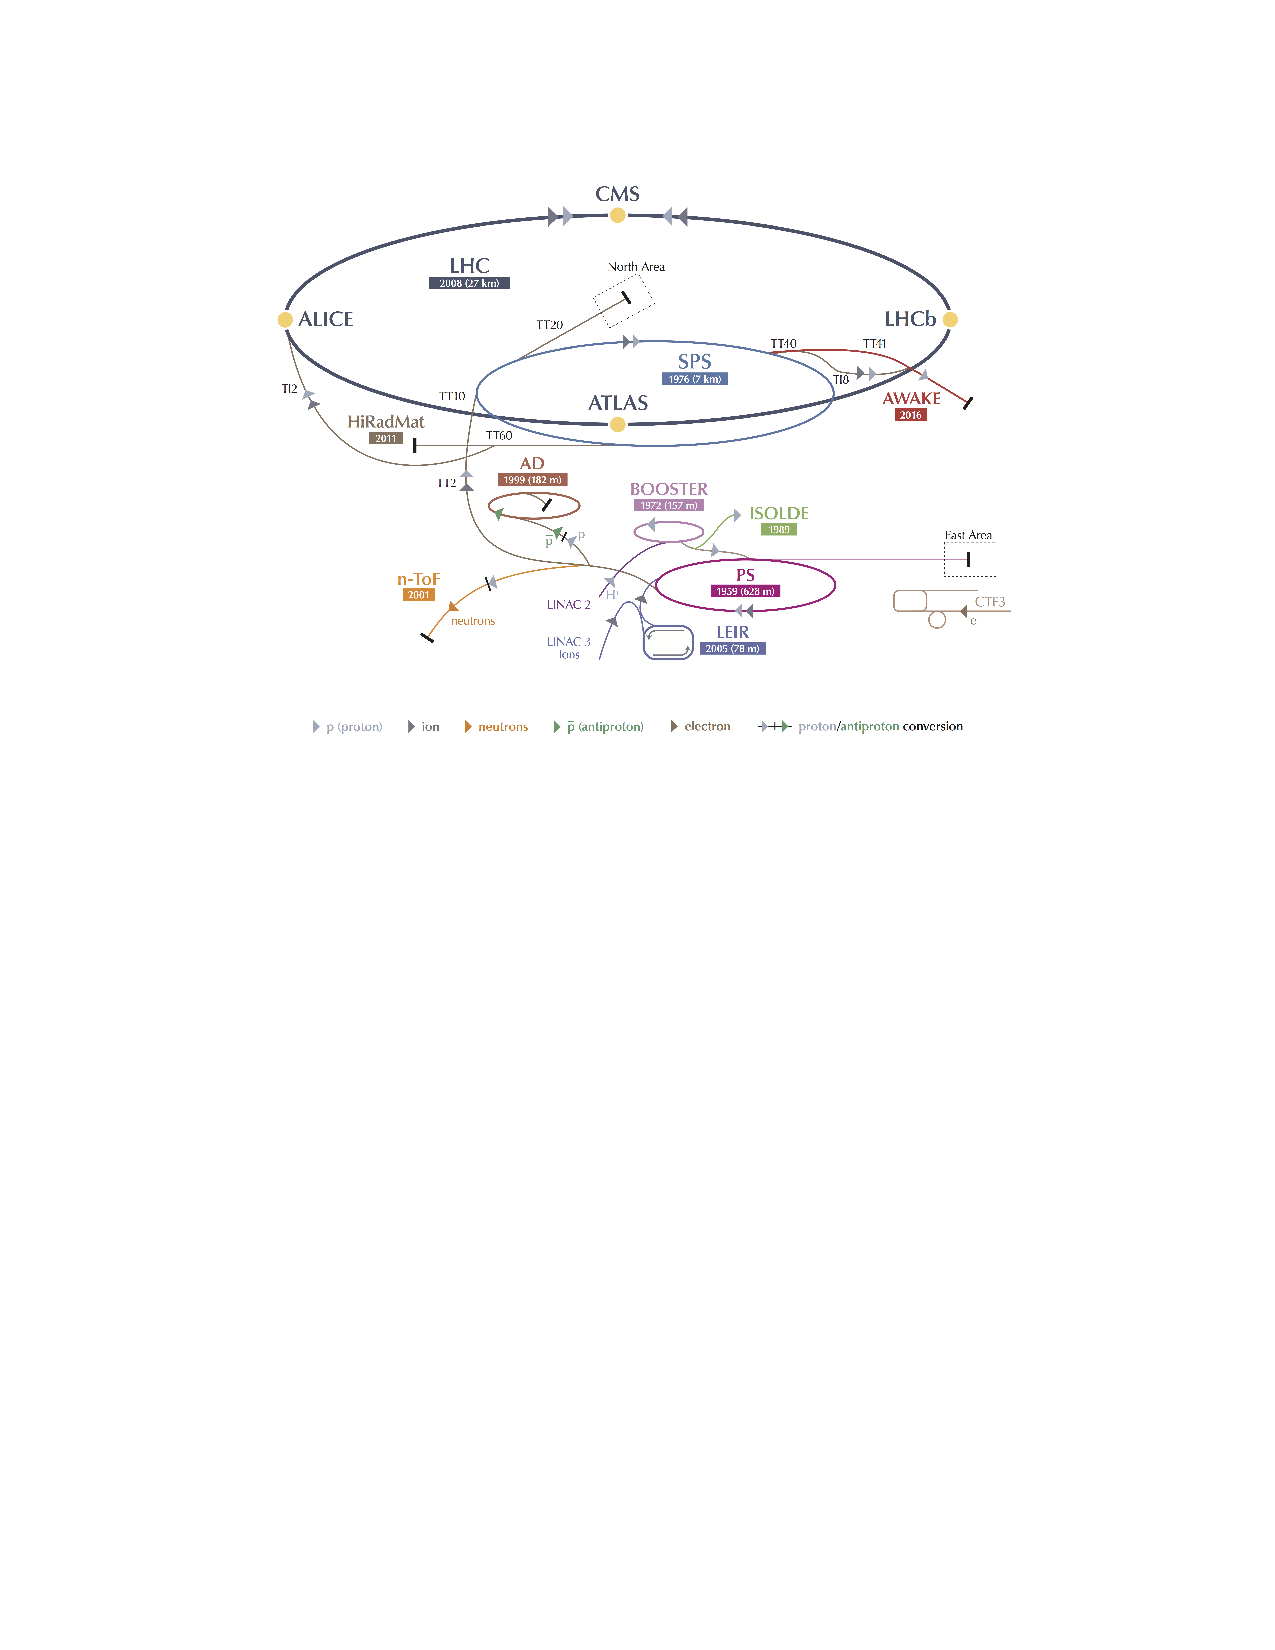
\includegraphics[width=.775\textwidth]{Collider/Figures/LHC_diagram.pdf}
  \caption{
    A schematic representation of the CERN accelerator complex. 
    The LHC (dark blue) is fed protons by a chain of intermediate accelerators, beginning with LINAC2 (light pink).
    Reprinted from the CERN Document Server~\cite{Mobs2018}. 
  }
  \label{fig:lhc}
\end{figure}


The LHC is a synchrotron containing 1232 superconducting NbTi dipole magnets measuring 15\unit{m} in length, each with a peak dipole field of 8.33\unit{T}. 
There are an additional 492 quadrupole magnets measuring 5-7\unit{m} in length which focus the beams in between the dipole magnets.
Due to space limitations in the tunnels, the beam pipes are magnetically coupled and the magnets share the same superfluid liquid helium cryostatic system required to achieve the 1.9\unit{K} temperature required to achieve the desired magnetic field strength and cool sufficient amount of power out of the system.

The number of events produced at the LHC is given by
\begin{equation}
  N(pp \rightarrow X) = \int dt L(t) \sigma(pp \rightarrow X),
\end{equation}
where $\sigma$ is the cross section of the process and $L$ is the instantaneous luminosity of the machine given by
\begin{equation}
  L = \frac{N_b^2 n_b f_{\text{rev}} \gamma}{4 \pi \epsilon \beta^*} \times F,
\end{equation}
where $N_b$ is the number of particles per bunch ($\mathcal{O}(10^{11})$),
$n_b$ is the number of bunches per beam,
$f_{\text{rev}}$ is frequency of revolution,
$\gamma$ is the Lorentz factor of the beam,
$\epsilon$ is transverse emittance of the beam,
$\beta^*$ is beta function of the beam at the collision point,
and $F$ is the geometric luminosity reduction factor due to the crossing angle at the interaction point.
The instantaneous luminosity decreases exponentially as a function of time due to $N_b$ and $n_b$ being reduced by collisions.
The LHC is designed to deliver an initial instantaneous luminosity of $\mathcal{O}(10^{34}) \percms$, achieved by having multiple inelastic proton-proton interactions per bunch crossing known as pileup.

As all known cross sections are time-independent, the total number of events is directly proportional to the integrated luminosity given by
\begin{equation}
  L_{\text{int}} = \int_0^T dt L(t) = L(0) \tau_L \left(1 - e^{-\sfrac{T}{\tau_L}} \right),
\end{equation}
where $T$ is the time since starting collisions,
$L(0)$ is the initial instantaneous luminosity,
and $\tau_L \approx 15\unit{h}$ the characteristic beam loss timescale for the LHC.
The total luminosity delivered by the LHC and recorded by CMS during the 2016 is shown in Figure~\ref{fig:lumi}.

\begin{figure}[htbp]
  \centering
  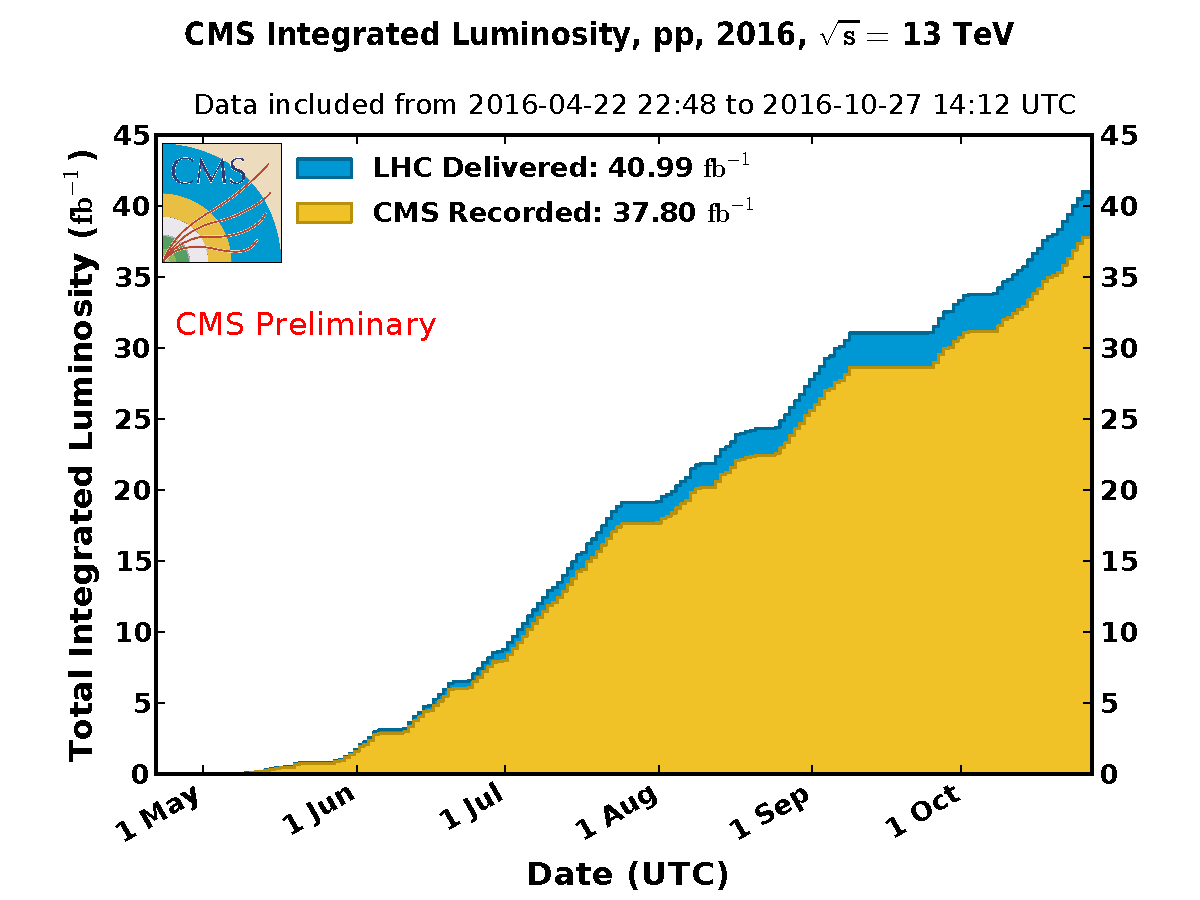
\includegraphics[width=0.75\textwidth]{Collider/Figures/lumi_2016.pdf}
  \caption{
    The total integrated luminosity of the LHC during proton-proton collisions during 2016 \cite{LumiTwiki}.
    While a total luminosity of 41\fbinv was collected, only a subset during which the detector operated well enough is used in this thesis. This corresponds to 36\fbinv of data.
  }
  \label{fig:lumi}
\end{figure}

\section{Collider Phenomenology}
\label{sec:collider_pheno}

The proton is a composite particle consisting of valence quarks, sea quarks, and gluons, collectively referred to as partons.
When colliding protons at the LHC, we are actually interested in the inelastic scattering of a pair of partons from the incident protons.
Each parton $a,b$ carries a fraction of the momentum of the incoming proton $x_{a,b}$ following the particle-dependent parton distribution functions (PDFs) $f_{a,b}$.
The differential cross section for $2\rightarrow N$ parton scattering process~\cite{Perelstein2010} is given by
\begin{equation}
  \text{d}\sigma \left(ab \rightarrow \{c_i\} \right) =
  \frac{(2\pi)^4}{2s} \left( \prod_i \frac{\text{d}^3 p_i}{(2\pi)^3} \right)
  \cdot \delta^4 \left(k_a + k_b - \sum_i p_i \right)
  \cdot \abs{ \mathcal{M} \left(ab \rightarrow \{c_i\} \right)}^2
\end{equation}
where $k_{a,b} = x_{a,b} \sqrt{s}$ are the momenta of the incoming partons, $\{p_i\}$ are the momenta of the outgoing partons $\{c_i\}$, and $\mathcal{M}$ is the matrix element of the process.

This parton level scattering, called the hard scattering process, is perturbatively calculable through standard QFT methods.
However, the hard scattering does not include any effects related to the PDFs of the incoming partons or the decay and hadronization of the outgoing partons into the final state particles (called the parton shower), both of which involve non-pertubative aspects of QCD.
Fortunately, the collinear factorization theorem~\cite{Collins1989} states that the probability of obtaining the final state $X(\Theta)$ from a hadron collision can be calculated as the product of the probability that specific partons $a,b$ are involved in the interaction, the probability for the hard scattering to produce outgoing partons $\{c_i\}$, and the formation of final state hadrons from these outgoing partons.
The factorization process is not unique and requires the choice of an arbitrary energy scale $\mu_F$, which defines a lower bound for interactions to be considered part of the hard scattering.

Including the effects from PDFs and parton showering (PS), the general cross section for $pp \rightarrow X(\Theta)$ is
\begin{align}
  \label{eqn:ppx}
  \frac{\text{d}\sigma}{\text{d}\Theta} \Big(pp \rightarrow X(\Theta) \Big) =
  \sum_{a,b} \int & \text{d} x_a f_a(x_a, \mu_F) \cdot \text{d} x_b f_b(x_b, \mu_F)  \nonumber \\
  & \times \text{d}\sigma \left(ab \rightarrow \{c_i\} \right)
  \times D \left( \{c_i\} \rightarrow X(\Theta) \right), 
\end{align}
where the sum is over the initial state partons and $D$ is the fragmentation function that describes parton shower process resulting in the observed final state.
The following sections discuss the simulation of the three main elements of Equation~\ref{eqn:ppx}: the parton distribution functions $f_a$, the hard scattering cross section $\text{d}\sigma$, and the parton shower and hadronization processes that contribute to the fragmentation function $D$.

\subsection{Parton Distribution Functions}

Due to soft collinear emissions from the partons, the behavior of the parton distribution functions depends on the factorization scale.
Denoting the gluon PDF as $g(x, \mu_F)$ and the PDF for quark flavor $i$ as $q_i(x, \mu_F)$, the analytic behavior of the PDFs is given by the DGLAP~\cite{Dokshitzer1977, Gribov1972, Altarelli1977} evolution equations
\begin{equation}
  \mu_F \frac{\text{d}}{\text{d} \mu_F} \begin{pmatrix} q_i(x, \mu_F) \\ g(x, \mu_F) \end{pmatrix}
  = \frac{\alpha_s}{2\pi} \int_{x}^{1} \frac{\text{d}y}{y}
  % {\Huge P}\left(\frac{x}{y}\right)
  \begin{pmatrix}
     P_{qq}\left(\sfrac{x}{y}\right) &  P_{qg}\left(\sfrac{x}{y}\right) \\
     P_{gq}\left(\sfrac{x}{y}\right) &  P_{gg}\left(\sfrac{x}{y}\right) 
  \end{pmatrix}
    \begin{pmatrix} q_i(y, \mu_F) \\ g(y, \mu_F) \end{pmatrix}
\end{equation}
where $y$ is the fraction of momentum carried by initial parton and the $P$ matrix elements are the splitting kernels defined by
\begin{equation}
  \begin{matrix}[l | l]
    P_{qq}(z) = \dfrac{4}{3} \left( \dfrac{1+z^2}{1-z} \right)
    & P_{qg}(z) = \dfrac{4}{3} \left( \dfrac{1+(1-z)^2}{z} \right)
    \\ \\ P_{gq}(z) = \dfrac{1}{2} \left( z^2 + (1+z)^2 \right)
    & P_{gg}(z) = 6 \left( \dfrac{1-z}{z} + \dfrac{z}{1-z} + z(1-z) \right) .
  \end{matrix}
\end{equation}

\begin{figure}[htbp]
  \centering
  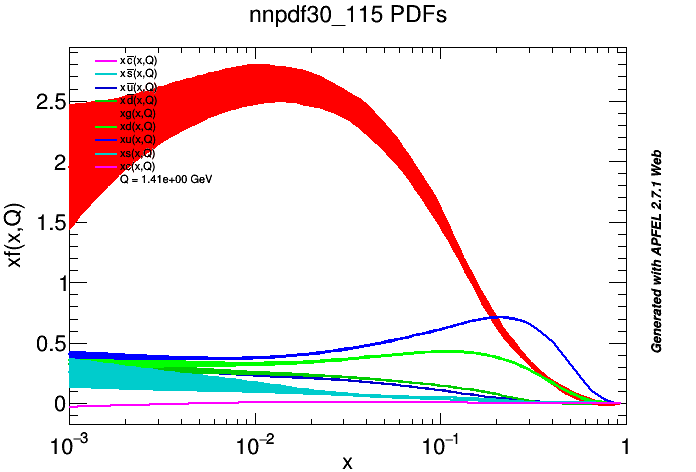
\includegraphics[width=0.625\textwidth]{Collider/Figures/nnpdf30_115_test.png}
  \caption{
    The various quark and gluon PDFs for the proton, as a function of momentum fraction $x$.
    The specific PDF set is the NNPDF3.0 118 NLO PDF set.
    % https://apfel.mi.infn.it/jobs
  }
  \label{fig:nnpdf}
\end{figure}

The DGLAP equations cannot be solved analytically at a fixed scale.
Instead, parameterized functional forms are fitted to data from many experiments.  
The results presented in this thesis use the NNPDF3.0 PDF set provided by the NNPDF collaboration~\cite{Ball2015}.
Figure~\ref{fig:nnpdf} shows the quark and gluon PDFs for the proton.
As $x \rightarrow 0$, the gluon fraction dominates while near $x \approx 0.3$, the up-quark fraction $u(x, \mu_F)$ approaches \sfrac{2}{3}, the down-quark fraction $d(x, \mu_F)$ approaches \sfrac{1}{3}, and the gluon and sea quark fractions approach zero.

\subsection{Hard Scattering}

The hard scattering process is simulated using Monte Carlo generators that sample events with probability proportional to the phase space and matrix element.
For the results contained in this thesis, the primary hard interaction is simulated using the MADGRAPH5 aMC@NLO generator~\cite{Alwall2014, Frederix2012}, which can simulate to leading order (LO) in EW vertices and up to next-to-leading order (NLO) in QCD vertices.

\subsection{Parton Shower}

The parton shower is a sequence of splittings where one outgoing parton $c_i$ emits a second soft and/or collinear particle $j$~\cite{Sjostrand2015}.
Each splitting has an associated splitting kernel $P_{c_i \rightarrow c_i j}(z)$, where $z$ is the momentum fraction carried by the initial parton.
The allowed QCD splittings are $q\rightarrow qg$, $g\rightarrow q \bar q$, and $g\rightarrow gg$ and the allowed QED splittings are $f\rightarrow f\gamma$ and $\gamma \rightarrow f \bar f$.
The kernels associated with these splittings are
\begin{equation}
  \begin{matrix}[l | l]
    P_{q\rightarrow qg}(z) = \dfrac{4}{3} \left( \dfrac{1+z^2}{1-z} \right)
    & P_{f \rightarrow f \gamma}(z) = Q_f^2 \left( \dfrac{1+z^2}{1-z} \right)
    \\ P_{g\rightarrow q \bar q}(z) = \dfrac{1}{2} \left( z^2 + (1-z)^2\right)
    & P_{\gamma \rightarrow f \bar f}(z) = N_C Q_f^2 \left( z^2 + (1-z)^2 \right) 
    \\ P_{g\rightarrow gg}(z) = 3 \left( \dfrac{(1-z(1-z))^2}{z(1-z)} \right)  & 
  \end{matrix}
\end{equation}
where $Q_f$ is the charge of the fermion and $N_C$ is the number of color states the fermion can occupy (3 for quarks and 1 for leptons).
The cross section of a splitting is given by
\begin{equation}
  \frac{\text{d}\sigma (ab\rightarrow \{c_i\}j)}{\text{d}\sigma (ab\rightarrow \{c_i\})}
  = P_{c_i\rightarrow c_i j}(z) \cdot \frac{\alpha_s}{2\pi} \cdot \frac{\text{d}\theta}{\theta} \cdot \text{d}z 
\end{equation}
where $\theta$ is the opening angle between $c_i$ and $j$.
These cross sections diverge as $\theta \rightarrow 0$ and $z \rightarrow 1$, meaning bare quarks producing many soft and collinear gluons.
Then, these gluons further split to $gg$ and $q\bar q$ pairs, which in turn emit even more soft and collinear gluons and photons.
This process continues until the energy of the outgoing partons reaches $\lqcd$ at which point hadronization occurs.
The final state particles from the shower of a single parton are often collimated into a narrow cone that is reconstructed as a single physics object called a jet.

\subsection{Hadronization}

The QCD potential between two quarks can be approximated as $ V(\vec r) \approx \kappa r$, where $\kappa$ has been measured to be approximately 1\unit{\GeVns/fm}.
The linear behavior of the potential is due to the attractive interactions between the gluons mediating the quark-quark interaction which confine the color field between the quarks into a tube 1 fm in diameter.
As the quarks separate, the energy contained in this gluon tube increases linearly until it exceeds the mass of a $q\bar q$ pair.
At this point, a new $q \bar q$ pair pops into existence through a quantum mechanical tunneling process, splitting the tube in two.
Due to the difference in quark masses, only up, down, and strange quarks are produced, in a 10:10:3 ratio.
This process continues until the energy of all the quarks have low enough energy to combine into stable hadrons.

The above procedure is a qualitative description of the Lund string model~\cite{Anderson1983}.
The Pythia event generator models hadronization using the Lund string model as well as the parton shower effects described in the previous section.
All results in this thesis use the Pythia 8.2 program~\cite{Sjostrand2015} to simulation the parton shower and hadronization processes. 

